\documentclass{article} 
\usepackage{phpn}
\usepackage{epsfig}
\usepackage{epstopdf}
\usepackage{graphicx}
\usepackage{algorithmic}



%------------------------------------------------------------------------------
\newcommand{\mydoctitle}     {GBT Proposal Life Cycle}
\newcommand{\mydocauthors}   {P. Marganian}
\newcommand{\mydocdate}      {\today}
\newcommand{\mydocnumber}    {1.0}
\newcommand{\mydocarchive}   {PH003}
\newcommand{\mydockeys}      {PH, PHT, proposals, sessions, projects, scheduling}

%------------------------------------------------------------------------------
% Document starts here with some standard preamble

\begin{document}

% Make header
\mydochead{\mydoctitle}{\mydocauthors}{\mydocdate}{\mydocnumber}
     {\mydocarchive}{\mydockeys}

\begin{abstract}
This memo describes the life cycles of Proposals for the Robert C. Byrd Green Bank Telescope.
\end{abstract}

\toc

\vspace{0.5in}
{\Large\bf History}
\begin{description}
\item [1.0] Original Draft (Marganian)
\end{description}

\clearpage


\section{Introduction}\label{intro}
oThe Robert C. Byrd Green Bank Telescope (GBT) has implemented a new Proposal Handling Tool (PHT) to
replace the previous tools for handling GBT proposals and preparing those proposals for scheduling. In addition
to replacing the previous proposal handling tools, the new tool is also integrated into both the GBT Dynamic
Scheduling System (DSS) and the NRAO-wide proposal submission and handling tools.

This document describes the proposal life cycle for GBT Proposals within the context of this new tool.

\section{Definitions}

\begin{itemize}
\item {\bf Proposal} - The scientific observing proposal, with its meta-data, which is submitted through the PST and which then may
eventually get scheduled on the telescope. 
\item {\bf Proposal Code} -  A unique identification code for the project. For science projects, this was assigned to the
project upon its proposal and is typically of the form GBTYYA-XX where YY is the year (e.g. 08), A
represents the semester to which the project was assigned (currently A, B, or C), and XX is a unique
number for that year and semester. A typical code is then GBT08A-059.
\item {\bf Semester} - A 6-month time period within a given year.  
\item {\bf Current Semester} - The semester which is ongoing.
\item {\bf Next Semester} - The semester following the Current Semester; most new Proposals aim to observe during the next semester.
\item {\bf Telescope Allocation Committe} (TAC) - Committee that allocates time for all NRAO telescopes.
\item {\bf GBT Dynamic Scheduling System} (DSS) - Software system used for scheduling the GBT.
\item {\bf Astrid } - Astronomer's integrated desktop; observer's tool for observing with the GBT.
\item {\bf GBT Scheduler} - The person who oversees the scheduling of the GBT.
\end{itemize}

\section{Overview}

\begin{figure}[h!]
\centering
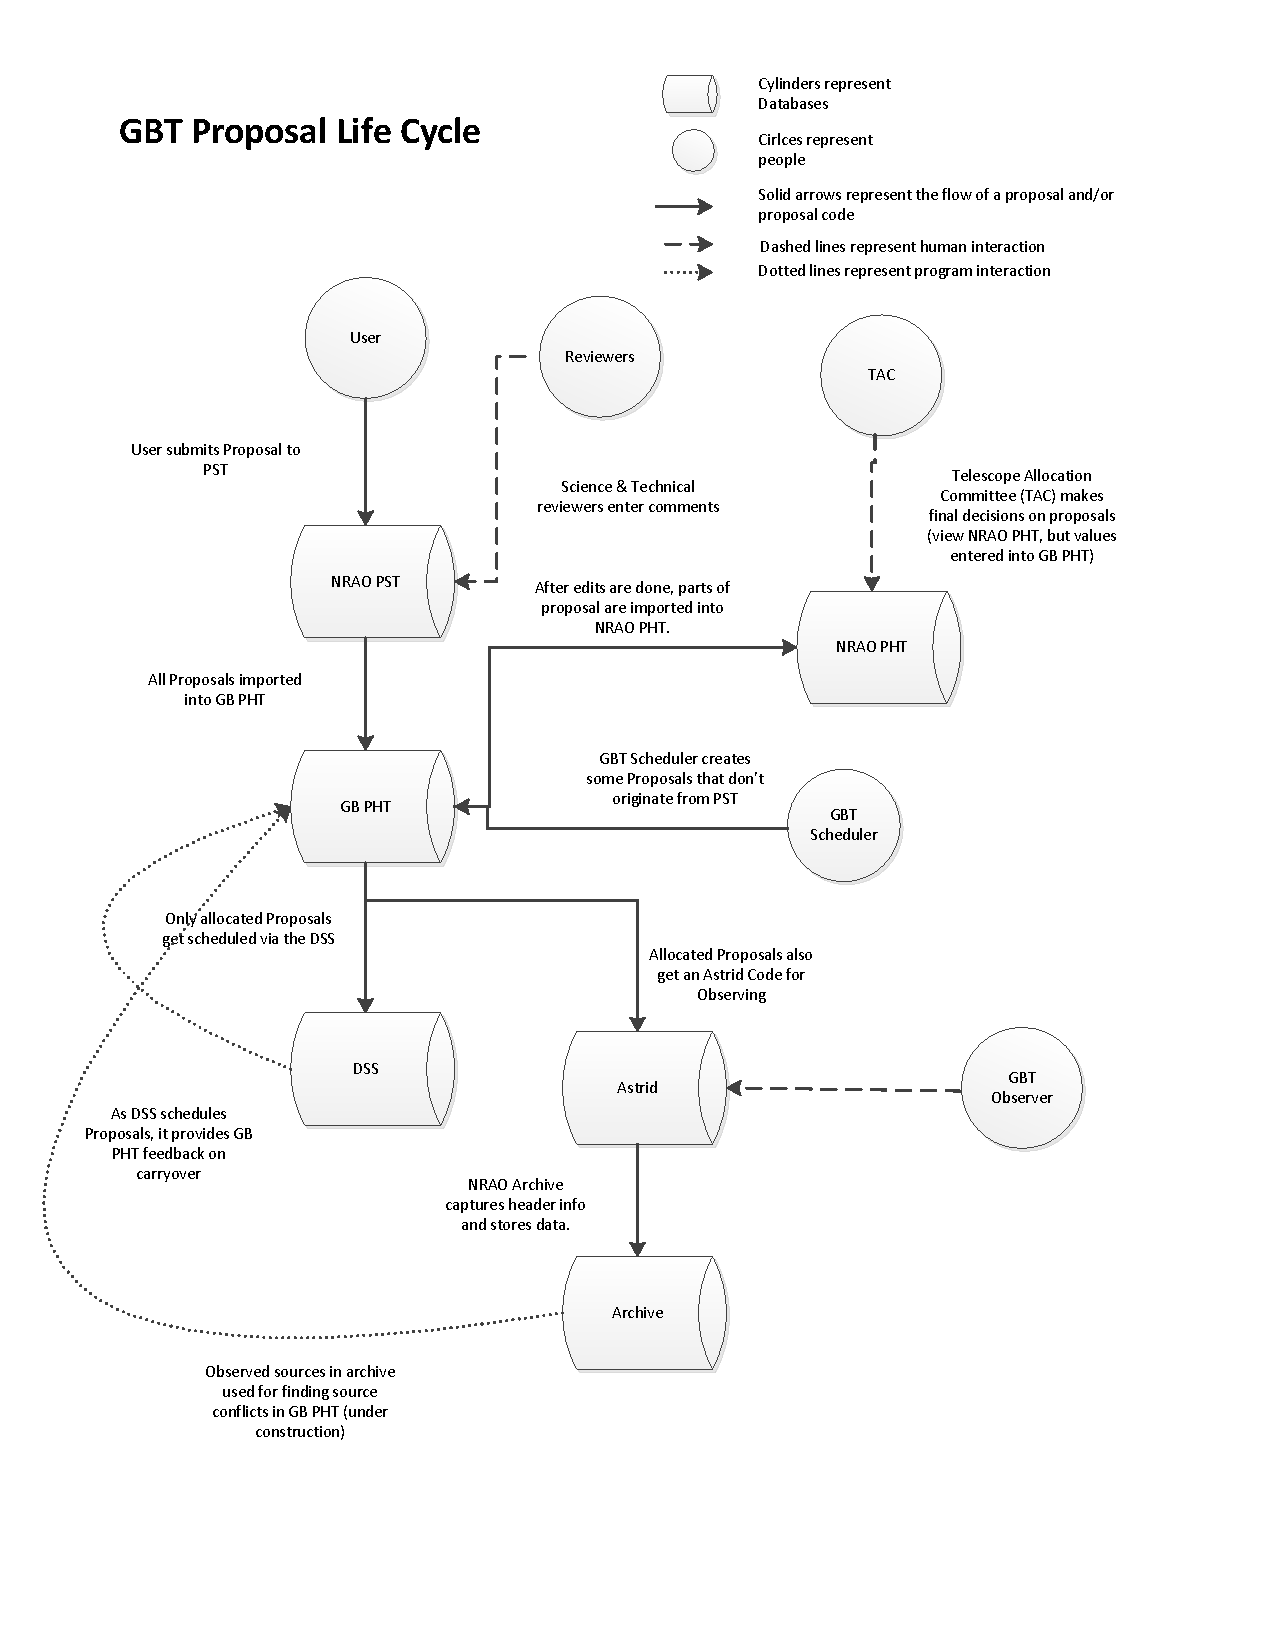
\includegraphics[width=0.8\textwidth]{ProposalLifeCycle.pdf}
\caption{GBT Proposal Life Cycle}
\label{proposal_life_cycle_image}
\end{figure}

Figure~\ref{proposal_life_cycle_image} shows the path(s) a GBT Proposal may take.
Here is a brief description of elements of this life cycle.  Note that details
are explained in other sections.

\begin{enumerate}
\item Scientist submits a Proposal into the NRAO Proposal Submission Tool
(PST) (Sec.~\ref{pst_sec}) before the submission deadline, which is the first day of the Current
Semester; thus this new Proposal may begin observing by Next Semester.  This
is the beginning of the Proposal's life cycle.
\item All new proposals for the Next Semester are imported into the GB PHT (Sec.~\ref{gb_pht_sec}).
\item Science Review Panels and Technical reviewers enter comments for each
Proposal in the PST.
\item Comments from reviewers are imported into GB PHT.
\item GBT Scheduler may optionaly add new Proposals directly into the GB PHT
\item GBT Scheduler edits Proposals in GB PHT
\item In preparation for the TAC meeting syncing is enabled between GB PHT and NRAO PHT (Sec.~\ref{nrao_pht_sec})
\item TAC meeting is held (about the middle of the Current Semester); TAC
feedback entered into GB PHT; changes propogated into NRAO PHT.  
\item GBT Proposals that have been allocated time are given a Dynamic
Scheduling System (DSS) (Sec.~\ref{dss_sec}) project so that they can be scheduled on the GBT, and
a corresponding Astrid Code (version of the Proposal code) so that they can
actually observe on the GBT (Sec.~\ref{astrid_sec}).
\item Once the Next Semester starts, Scientists start observing their
Proposals on the GBT:
Time Accounting in the DSS feedsback into the GB PHT so that the next TAC
knows how much 'carryover' still needs to be observed, and observations are
archived (Sec.~\ref{archive_sec}).
\item Resulting data from observations placed into the Archive.
\item Once a Proposal has observed enough of it's time on the GBT, it is
labeled as closed.  This is the end of the Proposal's life cycle.
\end{enumerate}

\section{Proposal Submission Tool}\label{pst_sec}

The NRAO Proposal Submission Tool (PST) is a package for creating and submitting proposals for 
NRAO telescopes. The PST has been used for GBT observing proposals since June 2005, 
VLA observing proposals since January 2006, and VLBA/HSA observing proposals since June 2008. 
The PST will eventually handle ALMA proposals.

The NRAO PST is a one-way interface into the GB and NRAO proposal handling tools.

\section{GB Proposal Handling Tool}\label{gb_pht_sec}

Once a GBT proposal is submitted through the NRAO Proposal Handling Tool and accepted for consideration, it is
imported into the Green Bank Proposal Handling Tool (GB PHT).  This is the tool which typically is used to allocate time, 
adjust sessions, and assign grades.  Information from this tool is also passed on to the NRAO Proposal Handling tool,
for record keeping, notification, and archiving purposes.


\section{NRAO Proposal Handling Tool}\label{nrao_pht_sec}

The NRAO Proposal Handling Tool processes the VLA and VLBA proposals in a manner similar to that of the GB PHT.  Additionally, it is the tool used for the NRAO TAC meeting, for sending of all dispositions to project investigators, and the primary archive for proposal information for NRAO telescopes.

\section{GBT Dynamic Scheduling System}\label{dss_sec}

The GBT DSS is used for scheduling observations on the GBT.  It is fully described within the NRAO GBT DSS memo series (ihttps://safe.nrao.edu/wiki/bin/view/GB/Dynamic/DynamicProjectNotes).

\subsection{DSS Projects and Sessions}

Once a Proposal has been allocated time by the TAC, it and its associated sessions and periods (if they exist) are 'exported' into the
GBT DSS.  That is to say, the PHT's Proposal is given an associated DSS Project.

The Proposal Code is used, without modification, for the DSS Project Code.

\subsection{Feedback to GB PHT}

As a DSS Project's Sessions are scheduled on the GBT, scientists manage their observing via Astrid (Sec.~\ref{astrid_sec}).  Utilitzing notes from the Operators Logs, the complex time accounting for these observations are determined in the DSS \cite{oneil11a}.  As the 'time remaining' for a given Project's Session decreases, the GBT Scheduler decides when and if the Project is 'complete', that is, when it should be done with its observations.

The DSS Project's 'time remaining' and 'complete' status are feed back
programatically to the GB PHT (contrary to Figure~\ref{proposal_life_cycle_image}, the GB PHT and DSS actually share the same database).  This is so that when the next cycle of new
proposals begins (the Next Semester becomes the Current Semester), any given
Proposal that has a corresponding DSS Project can be correctly taken into
account in the 'carryover'.  So, a DSS Project that is not 'complete' and
still has 'time remaining' will contribute to the 'carryover' of the LST
Pressures \cite{marganian12b}.

This feedback mechanism is further utilized through the use of the DSS
'lookahead simulations'.  Simulations form the core of the DSS Science
Algorithms.  A simulation can be run from the present day to the end of the
Current Semester, with reports detailing which sessions ended up completeing,
or how much 'time remaining' they may have.  These predictions can be leveraged by the GBT Scheduler by entering the results into the GB PHT Sessions' 'Next Semester' fields \cite{marganian12a}, thus ensuring a more accurate 'carryover' result for the LST Pressure plots presented to the TAC.

\section{Astrid}\label{astrid_sec}

Astrid is the tool used by scientists for managing their GBT observations.
When a GBT Proposal is allocated time by the TAC, it is given a corresponding
DSS Project (Sec.~\ref{dss_sec}) and Astrid Project Code. Unlike the DSS Project
Code, the GB Proposal Code is modified before it becomes an Astrid Project
Code:

\begin{itemize}
\item All "-" characters replaced with "\_".
\item If the Proposal Code does {\it not} begin with "T":
    \begin{itemize}
    \item If the Proposal Code is for VLBA, then "VLBA" is replaced with "AVLB".
    \item Othewise, simply append an "A" to the beginning of the Proposal Code.
    \end{itemize}
\end{itemize}

Note that previously, the PST 'legacy code' was being used for both DSS Proposal Codes, and Astrid Project Codes (i.e., BB240, etc.)

The Astrid Project Code is used in two significant ways:

\begin{itemize}
\item Scheduling Blocks (SB) - Observers make their actual observations by
submitting Scheduling Blocks via Astrid.  These SB's are managed via a
database, where they are organized via the Astrid Project Code.
\item Observation Data - Each time an observation is made via Astrid, the
Astrid Project Code must be chosen, as well as a 'session number' (no relation
to GB PHT and DSS essions).  The concatenation of these two values forms the
GBT M\&C Project Code, which in turn determines the directory where the
observation data is written to.  Also, the Astrid Project Code can be found in the data itself (FITS file headers).
\end{itemize}

\section{Archive}\label{archive_sec}

GBT data is being incorporated into the NRAO archive access tool (AAT).  The Astrid Project Code that is written in the data (FITS files) and forms part of the data directory discussed above is used for the Archive's 'Project Name'.  In addition, this same Astrid Project Code is  modified once again to form the Archive's 'Proposal Name', in a manner that restores it to the value that originated from the PST.    

\section{Proposal Code Summary}\label{pcode_summary_sec}

Here we give a brief summary of the uses of the proposal code from the birth
of the proposal, through to it's observations on the GBT.
\begin{itemize}
\item NRAO PST: Proposal Code originates
\item GB PHT: Proposal Code loses forward-slash character
\item DSS: Proposal Code reused without modification
\item Astrid: Proposal Code altered to become Astrid Project Code.
Concatenated with 'session number' to label data.
\item Archive: Astrid Project Code reused for 'Project Name';  Astrid Project Code modified for 'Proposal Name'
\end{itemize}

\subsubsection{Proposal Code Examples}

Example 1: GBT Proposal

\begin{itemize}
\item Scientist submits proposal at 2012-07-31 11:59:59.  It is assigned
Proposal Code GBT/13A-014
\item Proposals for semester 13A are imported on 2012-08-01 (first day of semester 12B).  Proposal code is changed to GBT13A-014.
\item Proposal is allocated time by TAC on 2012-10-13.  Proposals is given an associated DSS Project with Project Code GBT13A-014, and a corresponding Astrid Project Code of AGBT13A\_014.
\item Scientist observes Project after 13A starts (2013-02-01).  Their first observing session is labeled '01', so their data is stored in 'AGBT13A\_014\_01'.
\item Archive: Project Name = AGBT13A\_014, Proposal Name = GBT/13A-014
\end{itemize}

Example 2: VLBA Proposal

\begin{itemize}
\item Scientist submits proposal at 2012-07-31 11:59:58.  It is assigned
Proposal Code VLBA/13A-222
\item Proposals for semester 13A are imported on 2012-08-01 (first day of semester 12B).  Proposal code is changed to VLBA13A-222.
\item Proposal is allocated time by TAC on 2012-10-13.  Proposals is given an associated DSS Project with Project Code VLBA13A-222, and a corresponding Astrid Project Code of AVLB13A\_222.
\item Scientist observes Project after 13A starts (2013-02-01).  Their first observing session is labeled '01', so their data is stored in 'AVLB13A\_222\_01'.
\item Archive: Project Name = AVLB13A\_222, Proposal Name = VLBA/13A-222
\end{itemize}

\section{Exceptions}\label{exceptions_sec}

You can't have rules without exceptions.  Here's ours:  GBT Maintenance,
Shutdown and Testing.  These types of activities don't follow the same life
cycle path as 'astronomical' proposals.  These actually originate in the DSS,
and are later exported to the GB PHT.  They never are reviewed by the TAC, and
are treated differently when calculating LST Pressures \cite{marganian12b}.


\begin{thebibliography}{}
\bibitem[Marganian(2012)]{marganian12a}
  Marganian, Paul, 2012, ``PHT Time Accounting''
  PH/PN001.0
\bibitem[Marganian(2012)]{marganian12b}
  Marganian, Paul, 2012, ``PHT LST Pressures''
  PH/PN002.0
\bibitem[O'Neil(2011)]{oneil11a}
  O'Neil, Marganian, 2011, ``Time Accounting in the Green Bank Telescope Dynamic Scheduling
System''
  DS/PN011.3
\end{thebibliography}{}

\end{document}




















